\documentclass{article}

\usepackage{graphicx}
\usepackage{tabularx}
\usepackage{listings}
\usepackage{url}
\usepackage{footnote}
\usepackage{footmisc}
                                                                                                                       
\begin{document}

\title{ESCAPE Manual}
\author{Jan Van Campenhout \and Peter Verplaetse \and Jonas Maebe}

\maketitle

%%%%%%%%%%%%%%%%%%%%%%%%%%%%%%%%%%%%%%%%%%%%%%%%%%%%%%%%%%%%%%
\section{Introduction}
ESCAPE is an 
easy-to-use, highly interactive portable PC-based simulation environment
 aimed at the support of computer architecture education. The 
environment can simulate both a microprogrammed architecture and a 
pipelined architecture with simple pipeline. Both architectures are 
custom-made, with a certain amount of configurability. Other tools, such
 as a memory monitor, assembler/disassembler and analysis tools, such as
 on-the-fly generation of pipeline activity and usage diagrams, are 
integrated with the environment.

%%%%%%%%%%%%%%%%%%%%%%%%%%%%%%%%%%%%%%%%%%%%%%%%%%%%%%%%%%%%%%
\section{Architectural details}
The instruction set architecture is inspired by Hennessy and Patterson's
 DLX. The three distinguished types of instructions (I-type, R-type and 
J-type) are shown in Figure~\ref{fig:encoding}.

\begin{figure}
\centering
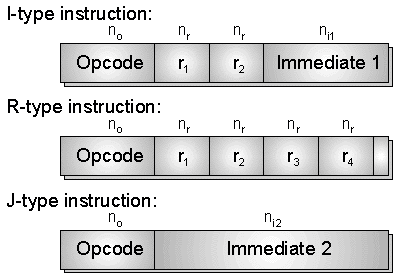
\includegraphics[width=5cm]{graphics/encoding.png}
\caption{ESCAPE instruction encoding.}
\label{fig:encoding}
\end{figure}

Contrary to the DLX architecture the size of the bitfields is not fixed,
 but depends on the maximum number of instructions and the size of the 
register file. All instructions have a 32-bit encoding, hence the length
 of the immediate fields ($n_{i1}$ and $n_{i2}$) can be derived from the bitfield sizes of the opcode and formals ($n_{o}$ and $n_{r}$):

\begin{quote}
$
n_{i1} = 32-n_{o}-2n_{r} \\
n_{i2} = 32-n_{o}
$
\end{quote}

R-type instructions can have up to 6 formals (assuming $n_{r}$ is 
sufficiently small). This can be useful for implementing more advanced 
operations in the microprogrammed architecture, a popular homework 
assignment.

%%%%%%%%%%%%%%%%%%%%%%%%%%%%%%%%%%%%%%%%%%%%%%%%%%%%%%%%%%%%%%
\subsection{Microprogrammed architecture}
The architecture consists of a control unit and a datapath. Figure~\ref{fig:micro}
shows a screenshot of the architecture as it appears in the simulator.

\begin{figure}
\centering
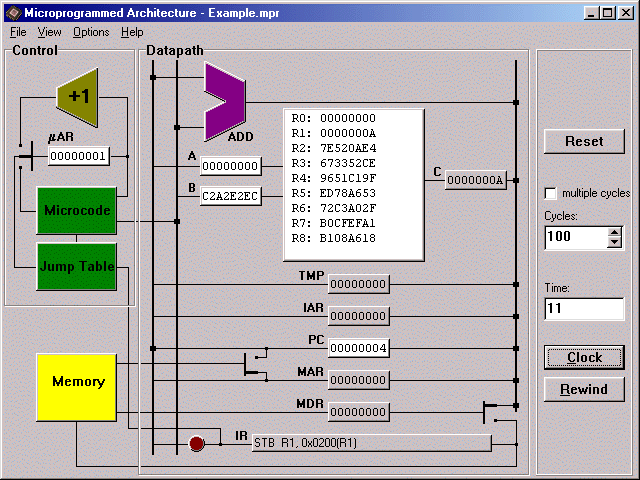
\includegraphics[width=11cm]{graphics/micro.png}
\caption{ESCAPE microprogrammed architecture.}
\label{fig:micro}
\end{figure}

The datapath consists of a register file, two read registers (\texttt{A}, \texttt{B}) and a write register (\texttt{C}), a memory interface with address (\texttt{MAR}), data (\texttt{MDR}) and instruction (\texttt{IR}) registers, a program counter (\texttt{PC}), a number of extra registers (typically \texttt{IAR} and a few temporary registers) and an ALU.  The different parts are connected by two input buses (\texttt{S1} and \texttt{S2})
 and a result bus. The ALU can perform a number of basic operations in a
 single cycle, as shown in the Table~\ref{table:microops}. A built-in comparator 
does zero and sign detection on the result.

\begin{table}
\begin{tabular}{l|l|l}
Operation 	& Result 			& Note  \\
\hline
ADD		& S1 $+$ S2			& add \\
SUB		& S1 $-$ S2			& subtract \\
RSUB		& S2 $-$ S1			& reverse subtract \\
MUL		& S1 $*$ S2			& multiply \\
DIV		& S1 $/$ S2			& divide \\
AND		& S1 \& S2			& bitwise and \\
OR		& S1 $|$ S2			& bitwise or \\
XOR		& S1 \^{} S2			& bitwise exclusive or \\
SLL		& S1 $<<$ S2			& shift left logical \\
SRL		& S1 $>>>$ S2			& shift right logical \\
SRA		& S1 $>>$ S2 			& shift right arithmetic \\
S1		& S1				& pass S1 \\
S2		& S2				& pass S2 \\
S2S1		& S2[15:0] $<<$ 16 $|$ S1[15:0]	& for the LIH instruction
\end{tabular}
\caption{ALU operations avaiblable in the microprogrammed architecture.}
\label{table:microops}
\end{table}

The memory interface can load and store bytes, halves (16 bit) or words (32 bit), with adjustable access time. Both
instructions and data are stored in the same memory (von Neumann architecture).

The control unit is microprogrammed. The microcode address is kept in a special register (\texttt{uAR}). During each cycle \texttt{uAR}
 is either incremented or replaced with a new value (i.e. a jump to a 
new microinstruction). Typical jump conditions are: memory busy, ALU 
output zero, ALU output negative and interrupt pending. The jump address
 is either stored in the microcode, or read from a jump table (indexed 
by the opcode field in \texttt{IR}). The latter is useful for instruction decoding. The number of jump tables is adjustable from 1 to 4.

%%%%%%%%%%%%%%%%%%%%%%%%%%%%%%%%%%%%%%%%%%%%%%%%%%%%%%%%%%%%%%
\subsection{Pipelined architecture}
Both the control unit and the datapath are pipelined into the five 
traditional stages: IF (instruction fetch), ID (instruction decode), EX 
(execute and effective address calculation), MEM (memory) and WB (write 
back), as can be seen in Figure~\ref{fig:pipe}.

\begin{figure}
\centering
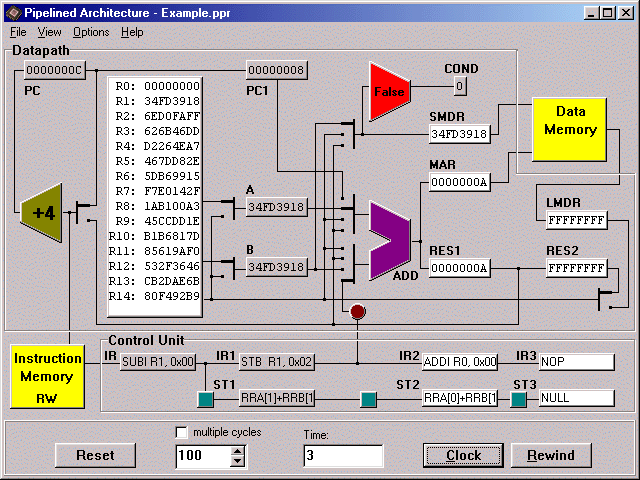
\includegraphics[width=11cm]{graphics/pipe.png}
\caption{Overview of the piplined architecture form}
\label{fig:pipe}
\end{figure}

Because there are at least three cycles between reading the register file and write back, a forwarding mechanism is
implemented to prevent the pipe from unnecessary stalling. The register file is read in the ID stage, but written during
the WB stage. Write through is explicit by the use of multiplexers.

The EX stage consists of an ALU and a comparator. The ALU can perform
 the same operations as the one for the microprogrammed architecture. 
During the execution of a branch the comparator evaluates the branch 
condition while the ALU calculates the effective address. Depending on 
the settings of the simulator the two instructions following the branch
can be executed (i.e., a \emph{double} delay slot), nullified (no delay slot), or only the instruction in the IF stage is
nullified (single delay slot).

There are two separate memory interfaces: one for instructions 
and one for data (Harvard architecture). The instruction memory access 
time is fixed (single cycle access); the data memory access time is 
adjustable from 1 to 9 clockcycles. Access to the data memory occurs 
during the MEM stage. 

%%%%%%%%%%%%%%%%%%%%%%%%%%%%%%%%%%%%%%%%%%%%%%%%%%%%%%%%%%%%%%
\section{Form overview}
The application consists of several forms or windows. The most important forms are:

\begin{itemize}
\item Main Form
\item Configuration Form
\item Microprogrammed Architecture Form
\item Microcode \& Jump Tables Form
\item Pipelined Architecture Form
\item Pipeline Functionality Form
\item Pipeline Diagrams
\item Instruction Memory Form
\item Data Memory Form
\item Breakpoints Form
\end{itemize}

The forms will be discussed in more detail in the following sections. Most forms have menus.  Additionally, the right mouse
button can be used to perform most actions from a contextual menu.

%%%%%%%%%%%%%%%%%%%%%%%%%%%%%%%%%%%%%%%%%%%%%%%%%%%%%%%%%%%%%%
\section{Main Form}
After launching the simulation environment the main form appears. On the right side of the form are three buttons. By
clicking on these buttons you can launch the simulator for the microprogrammed or the pipelined architecture, or
configure both architectures.

Click on the close icon of the window to exit the application. If the
 current configuration has changed but has not been saved yet, the user 
is asked to save the configuration first.

%%%%%%%%%%%%%%%%%%%%%%%%%%%%%%%%%%%%%%%%%%%%%%%%%%%%%%%%%%%%%%
\section{Configuration Form}
The configuration form can be used to configure both architectures. The configuration is stored in a file with the \texttt{.ecf} extension.
When starting ESCAPE, the application first looks for \texttt{escape.ecf}. If this file is not found, it searches for any \texttt{*.ecf}
 file. When such a file is found, it is loaded as the default 
configuration. If no files match, no default configuration is loaded.

The configuration form consists of 4 pages: general options, instruction encoding and two architecture specific
forms. You can switch from one page to another by clicking on the tabs on the bottom of the form.

%%%%%%%%%%%%%%%%%%%%%%%%%%%%%%%%%%%%%%%%%%%%%%%%%%%%%%%%%%%%%%
\subsection{General options}

\begin{description}
\item[ALU Operations] MULT and DIV operations can be disabled, since it is not realistic for those operations to be executed in a single cycle.
\item[Comparator Operations] A minimal or complete set of 
comparator operations can be selected. The minimal set consists of only 
two operations: equal and less than. The complete set consists of all 6 
operations (equal, not equal, less than, greater than, less than or 
equal and greater than or equal).
\item[Sign Extend] Sign extension can be done to bytes, halves or words, or to words only.
\item[Memory Operations] Memory operations can be done with byte, half and word resolution, or word only resolution.
\item[Memory Size] The data memory size can be set from 64 to 
32768 bytes. The code memory size (pipelined architecture) or default 
code range (microprogrammed architecture) can be set from 64 to 32768 as
 well.
\end{description}

%%%%%%%%%%%%%%%%%%%%%%%%%%%%%%%%%%%%%%%%%%%%%%%%%%%%%%%%%%%%%%
\subsection{Instruction encoding}
The \emph{number of opcodes} can be set from 16 to 256. The \emph{number of registers} in the register file is
configurable from 4 to 256. Changing these two numbers influences the size of the immediates and the number of formals
that can be used for R-type instructions. Note that register R0 always contains the value `0' and any write operation to
this register will be ignored. Therefore, the actual number of registers available is one less than the value specified.

For each instruction one must specify:
\begin{description}
\item[The Opcode] Alphanumeric characters without spaces.
\item[The Instruction Type] R-, I- or J-type.
\item[The Mnemonic Representation] The textual representation 
of the operands. The formals r1-r6 will be replaced by actuals (with 
capital R). Use `i' or `j' to represent immediates. Note that both `i' 
and `j' can be used for both I-type and J-type instructions: with `i' 
the immediate is represented as an absolute integer; with `j' the 
immediate is interpreted as a PC-relative address (relative to the 
address of the next instruction) and labels are used when possible.
\end{description}

\subsection{Microprogrammed architecture}

\begin{description}
\item[Microcode Memory] The microcode size can be set from 2 to 1024 lines. The width of the constant field is configurable from 0 to 32 bits.
\item[Register File Operations] Specify which formals should be read in registers \texttt{A} and \texttt{B} during an RR operation.
Checkmark the additional operations that can be performed (RAF: read formal into \texttt{A}; RBF: read formal into \texttt{B};
RAA: read actual into \texttt{A}; RBA: read actual into \texttt{B}; WF: write formal; WA: write actual).
\item[Jump Tables] Set the number of tables from 1 to 4.
\item[Extra Registers] Enter the names of the extra organizational registers. 
\end{description}

%%%%%%%%%%%%%%%%%%%%%%%%%%%%%%%%%%%%%%%%%%%%%%%%%%%%%%%%%%%%%%
\subsection{Pipelined architecture}

\begin{description}
\item[Register File Reading] Since instruction
decoding is on the critical path and register file accesses are slow as well, it is not realistic when the formals to be
read during the ID stage depend on the instruction that gets decoded at the same time. When register file reading is set
to \emph{Instruction Independent}, register \texttt{A} (\texttt{B}) is always loaded with formal 1 (2).

\item[Stall Control] Stalling of the different
stages is controlled independently. This may appear strange to those who are used to always having the pipe stalling
upstream. Therefore, stall control can be set to \emph{Unconditionally Stall Upstream} to achieve the latter.
\end{description}

\subsection{Menu items}

\begin{description}
\item[File $\to$ New File] Discard all settings.
\item[File $\to$ Open File] Read settings from a file.
\item[File $\to$ Save File] Write the current settings to a file. The user is prompted for a file name when no name has been specified.
\item[File $\to$ Save File As]Similar to the previous menu, but the user is always prompted for a file name.
\item[File $\to$ Hide Form] Hides the configuration form and displays the main form again. The same can be achieved by clicking on the window close icon.
\item[Help $\to$ About]Shows the about box.
\end{description}

\section{Microprogrammed Architecture Form}
The microprogrammed architecture form shows most organizational elements of this architecture. If not all registers in
the register file are visible, click on the register file to show a blinking cursor. Use the cursor keys to walk through
the registers. The position of the multiplexers and the bus sources are visualized by thick black lines. Registers that
have a gray background are disabled (and will keep their content during the next clock cycle). Registers with a white
background will be update during the next cycle.

By clicking on the wires that interconnect the different elements a 
pop-up box appears that shows the driver and current value of that wire.

On the right of the form are a few buttons and boxes to control the simulation. A click on the \textbf{Reset} button
results in initialization of the architecture. Click on the \textbf{Clock} button to simulate one or multiple
clockcycles. A click on the \textbf{Rewind} button will rewind the clock. Note that the clock can not be rewound for more
than 1024 cycles. If the \textbf{multiple cycles} box is checkmarked, the number of cycles specified in the \textbf{Cycles}
box will be simulated or rewound. You can also enter a new value in the \textbf{Time} box to simulate or rewind
clockcycles.

When simulating more than one cycle, the simulation will be interrupted when a breakpoint condition is met or when a
memory access violation occurs.

%%%%%%%%%%%%%%%%%%%%%%%%%%%%%%%%%%%%%%%%%%%%%%%%%%%%%%%%%%%%%%
\subsection{Menu items}

\begin{description}
\item[File $\to$ New Project] Clear the memory and discard all settings
\item[File $\to$ Open Project] Load the settings from a
 file. This will automatically load data and instruction memory modules,
 and microcode. Since code and data memory are physically the same (von 
Neumann architecture), part of the data memory is overwritten with the 
code memory. This allows the user to manually edit the instruction 
memory files.
\item[File $\to$ Save Project] Saves the settings to a file. The instruction and data memory modules, and the microcode will be saved as well.
\item[File $\to$ Save Project As] Similar to the previous menu, but the user is prompted for a project file name.
\item[File $\to$ Set Trace File] Before trace file generation can be enabled (see the \textbf{Options $\to$ Generate Trace File} item), a trace file must be set first. Warning: this will erase the selected trace file.
\item[File $\to$ Exit] Exits the simulator and shows the main form again. The user is prompted to save the project if necessary.
\item[View $\to$ Instruction Memory] Shows the instruction view of the main memory.
\item[View $\to$ Data Memory] Selecting this item shows the data view of the main memory.
\item[View $\to$ Microcode] By clicking on this item the microcode and jump tables form is displayed.
\item[View $\to$ Breakpoints] Click on this item to display the breakpoints form.
\item[Options $\to$ Generate Trace File] After setting a trace file (with \textbf{File $\to$ Trace File}) this menu item becomes enabled. Click on it to generate a trace file while simulating. Each time the \texttt{PC}
 register is changed, a new line is added to the trace file. This may 
not work properly with self-modifying code. By clicking on the \textbf{Options $\to$ Generate Trace File} item again, the checkmark is removed and trace file generation is disabled.
\item[Options $\to$ Enable Rewind] To speed up simulation the rewind option can be disabled. It can be enabled at any time -- the \textbf{Rewind} button will be enabled as soon as you simulate more clock cycles.
\item[Options $\to$ Memory Access Time] Select this 
item to set the memory access time to a value from 1 to 9 cycles. The 
default value is 4 cycles. The architecture will automatically be reset 
whenever the memory access time is altered.
\item[Help $\to$ About] Shows the about box.
\end{description}

%%%%%%%%%%%%%%%%%%%%%%%%%%%%%%%%%%%%%%%%%%%%%%%%%%%%%%%%%%%%%%
\section{Microcode \& Jump Tables Form}
This form can be used to define the functionality of the microprogrammed architectures. The form consists of two pages: a
\textbf{Microcode} page and a \textbf{Jump Tables} page. You can switch from one page to another by clicking on the tabs on the bottom of the form, or by clicking on one of the \textbf{View} menu items.

%%%%%%%%%%%%%%%%%%%%%%%%%%%%%%%%%%%%%%%%%%%%%%%%%%%%%%%%%%%%%%
\subsection{Microcode}
The microcode is represented as a table. Each row of the table corresponds to a microinstruction. Each row in this
table has to be seen as a set of parallel instructions at the microcode level, and consists of the following items:

\begin{description}
\item[uAR ]This is the microcode address. 
\item[Label] Since the microcode address can change when inserting or deleting rows, labels are used to specify jump addresses
in the microcode. Enter a label (alphanumeric sequence without whitespace) here to identify the microinstruction.
\item[ALU] The functionality of the ALU when executing this microcode instruction. Possible values are: (empty --
 no operation), ADD, SUB, RSUB, AND, OR, XOR, SLL, SRL, SRA, S1, S2, 
S2S1 and MUL and DIV when they are enabled on the configuration form.
\item[S1] The source of bus S1. Possible values are: (empty --
 no source), A, Const, PC, MAR, MDR, IR and the extra organizational 
registers added on the configuration form. All sources are 
organizational registers, with the exception of Const, which is a number
 coded in the microinstruction, and IR, which is really a sign extended 
version of the immediate coded in the current macroinstruction. 
\item[S2] The source of bus S2. Possible values are: (empty -- no source), B, Const, PC, MAR, MDR, IR and the extra organizational registers added on the configuration form.
\item[Dest] The destination of the ALU. Possible values are: (empty -- no destination), C, PC, MAR, MDR and the extra organizational registers added on the configuration form.
\item[ExtIR] The size to which the immediate coded in the 
macroinstruction should be extended. Depending on the configuration, the
 possible values are: (empty), Byte, Word and Half, or (empty) or Word. 
When (empty) is selected, no
extension occurs, and the full 32 bit of the instruction register is 
used.
\item[Const] The constant coded in the microinstruction. The 
number of bits can be set on the configuration form. Enter the value in 
decimal (signed or unsigned), or in hexadecimal. In the latter case the 
number must start with "0x".
\item[JCond] This field determines which microinstruction will be executed next. The possible values are shown in Table~\ref{table:jcond}.
\item[Adr] The label of the microinstruction to be executed next when the jump condition evaluates to true.
\item[Mem] The functionality of the memory interface. Depending
 on the settings on the configuration form, the possible values are: 
(empty -- no operation), RW and WW or (empty), RB, RH, RW, WB, 
WH, WW. The first character indicates read (R) or write (W), the second 
character indicates the width of the memory access: byte (B), half (H -- 16 bit) 
or word (W -- 32 bit).
\item[MAdr] The source of the memory address for read or write operations. Either (empty -- defaults to MAR), MAR or PC.
\item[MDest] The destination register for memory read operations. Possible values are: (empty -- defaults to IR), MDR or IR.
\item[Regs] The functionality of the register file. The 
possible values depend on the settings on the configuration form and are
 explained in Table~\ref{table:regs}
\end{description} 

\begin{table}
\begin{minipage}{6cm}
\begin{tabular}{l|l}
Value		& Result \\
\hline
(empty)		& uAR := uAR+1 \\
True		& uAR := Adr (Adr is coded in the microinstruction) \\
EQ		& uAR := Adr when Result(ALU) $=$ 0 \\
NE\footnote{These values are only available when the complete set is selected for the comparator on the configuration form.\label{foot:completecomp}}
		& uAR := Adr when Result(ALU) $\neq$ 0 \\
LT		& uAR := Adr when Result(ALU) $<$ 0 \\
GT\footref{foot:completecomp}
		& uAR := Adr when Result(ALU) $>$ 0 \\
LE\footref{foot:completecomp}           
		& uAR := Adr when Result(ALU) $\leq$ 0 \\
GE\footref{foot:completecomp}           
		& uAR := Adr when Result(ALU) $\geq$ 0 \\
MBusy		& uAR := Adr when the memory is busy \\
$Jump_{n}$	& uAR := Address(Jump Table n)
\end{tabular}
\caption{Overview of the available jump conditions in the microarchitecture (JCond).}
\label{table:jcond}
\end{minipage}
\end{table}

\begin{table}
\begin{tabular}{l|l}
Value	& Function \\
\hline
RR	& Read formals into registers \texttt{A} and \texttt{B} \\
$RAF_{n}$	& Read formal n into register \texttt{A} \\
$RBF_{n}$	& Read formal n into register \texttt{B} \\
$WF_{n}$	& Write register \texttt{C} into formal n \\
$RAA_{n}$	& Read actual n into register \texttt{A} \\
$RBA_{n}$	& Read actual n into register \texttt{B} \\
$WA_{n}$	& Write register \texttt{C} into actual n
\end{tabular}
\caption{Overview of the available register file operations in the microarchitecture (Regs).}
\label{table:regs}
\end{table}

When editing a field whose possible values consist of a predefined list,
the editor will show the possible completions for what has already been
typed. If the final value is invalid, the previous value will be restored.

In addition to the default overwrite mode, there is also an insert mode. Toggle from one to another with the \textbf{Insert} key
or by toggling its value in the pop-up menu at the bottom of the window. In insert mode an empty row is inserted whenever
the user hits the \textbf{Enter key}, and when pasting the rows are inserted instead of being overwritten.

%%%%%%%%%%%%%%%%%%%%%%%%%%%%%%%%%%%%%%%%%%%%%%%%%%%%%%%%%%%%%%
\subsection{Jump Tables}
The jump tables form is a table with the opcodes in the first column and
 destinations fields for the jump tables in other columns. When the 
JCond field of the current microinstruction has a value of $Jump_{n}$, the next microinstruction to be executed is determined by the row in jump table n indexed by the opcode portion of \texttt{IR}. 

%%%%%%%%%%%%%%%%%%%%%%%%%%%%%%%%%%%%%%%%%%%%%%%%%%%%%%%%%%%%%%
\subsection{Menu items}

\begin{description}
\item[File $\to$ New File] Discard all data.
\item[File $\to$ Open File] Read microcode and jump 
tables from a file. Since all files are ASCII, they can be edited with a
 simple editor (such as Notepad). Because labels are used for jumps, the
 microcode address does not have to be updated manually: after loading 
the microcode the addresses are renumbered automatically.
\item[File $\to$ Save File] Write the data to a file. The user is prompted for a file name when no name has been specified.
\item[File $\to$ Save File As] Similar to the previous menu, but the user is always prompted for a file name.
\item[File $\to$ Hide Form] Hides the microcode form, 
which can also be achieved by clicking on the window close icon. Note 
that the form still exists, therefore the user is not yet prompted to 
save any data that may have been modified.
\item[Edit $\to$ Cut] Only enabled when editing the 
microcode page. After selecting one or more rows, select this menu item 
to cut the rows to the clipboard.
\item[Edit $\to$ Copy] Only enabled when editing the microcode page. Select this menu item to copy rows to the clipboard.
\item[Edit $\to$ Paste] Only enabled when editing the microcode page. Inserts or overwrites the rows cut or copied to the clipboard.
\item[Edit $\to$ Delete] Only enabled when editing the microcode page. Deletes the selected rows.
\item[Edit $\to$ Select All] Only enabled when editing the microcode page. Selects all rows.
\item[Edit $\to$ Copy Opcodes] Only enabled when 
editing the jump tables page. After selecting a certain jump table field
 and selecting this menu item, all fields of the jump table are filled 
with the opcode names as labels. This can be useful when using a jump 
table for the decoding of instructions.
\item[Edit $\to$ Fill] Only enabled when editing the 
jump tables page. First the user is prompted for a value, then all the 
selected fields are filled with this value.
\item[Edit $\to$ Dropdown Mode] Toggles between dropdown and edit mode.
\item[View $\to$ Microcode] Show the microcode page.
\item[View $\to$ Jump Tables] Show the jump tables page.
\item[View $\to$ Base] Set the base for viewing the Const field to either Unsigned Hexadecimal, Unsigned Decimal or Signed Decimal.
\item[Assemble $\to$ Assemble] Since labels are used 
for jumps, an assembly routine is required to lookup all the microcode 
addresses the labels refer to. The assemble routine is automatically 
invoked when loading or saving the microcode, and before simulating, 
therefore it is never necessary to assemble manually. It can however be 
useful to check for errors while writing microcode.
\item[Help $\to$ About] Shows the about box.
\end{description}

%%%%%%%%%%%%%%%%%%%%%%%%%%%%%%%%%%%%%%%%%%%%%%%%%%%%%%%%%%%%%%
\section{Pipelined Architecture Form}
The pipelined architecture form is very similar in use to the 
microprogrammed architecture form. The register file can be scrolled 
with the cursor keys, the multiplexer positions are visualized by thick 
black lines and registers with a gray background are disabled. Pop-up 
boxes to show the driver and current value of wires are also available 
here. The interface (Clock, Reset and Rewind buttons, etc.) is also 
similar.

%%%%%%%%%%%%%%%%%%%%%%%%%%%%%%%%%%%%%%%%%%%%%%%%%%%%%%%%%%%%%%
\subsection{Menu items}
Most menu items are identical to those of the microprogrammed architecture form. The \textbf{View $\to$ Microcode} item is replaced by \textbf{View $\to$ Pipeline Functionality}, and a few additional menu items exist.

\begin{description}
\item[View $\to$ Pipeline Functionality] Clicking on this item the pipeline functionality form is displayed.
\item[View $\to$ Enable Pipeline Diagrams] Click on this item to enable the pipeline diagrams. This will slow down the simulation a little.
\item[View $\to$ Pipeline Activity Diagram] Displays the pipeline activity diagram.
\item[View $\to$ Pipeline Usage Diagram] Displays the pipeline usage diagram.
\item[Options $\to$ Enable Forwarding] Checkmark to 
enable forwarding. When forwarding is disabled, explicit write-through 
of the register file is still enabled, and stalls of the EX-stage will 
occur instead of forwarding. Forwarding is enabled by default.
\item[Options $\to$ Delayed Branching] Use this menu item to set the delay slot size to either No Delay Slot, Single Delay Slot or Double Delay Slot.
\item[Options $\to$ Data Memory Access Time] The 
default data memory access time is 3 clockcycles, but can be set from 1 
to 9 cycles. The architecture will automatically be reset whenever the 
memory access time is altered.
\end{description}

%%%%%%%%%%%%%%%%%%%%%%%%%%%%%%%%%%%%%%%%%%%%%%%%%%%%%%%%%%%%%%
\section{Pipeline Functionality Form}
This form is the counterpart of the microcode and jump tables form for 
the pipelined architecture. The pipeline functionality is represented in
 tabular form as well. For each opcode a number of items must be 
specified:

\begin{description}
\item[A Formal] The formal to be read in register \texttt{A} during the ID stage. Possible values are: (empty --
 no register is read), 1, 2 and 3. When register file reading is set to 
instruction independent on the configuration form, register \texttt{A} is always loaded with formal 1.
\item[B Formal] The formal to be read in register \texttt{B}. When register file reading is set to instruction independent, register \texttt{B} is always loaded with formal 2.
\item[C Formal] The formal to be written during the WB stage. Possible values are: (empty -- no write-back occurs), 1, 2 and 3.
\item[S1] The source for the first ALU operand. The possible values are: (empty -- defaults to A), A or PC1.
\item[S2] The source for the second ALU operand. The possible values are: (empty -- defaults to B), B or IR.
\item[IR Extend] The size to which the immediate coded in the 
macroinstruction should be extended. Depending on the configuration, the
 possible values are: (empty), Byte, Word and Half, or (empty) or Word. 
When (empty) is selected, no
extension occurs, and the full 32 bit of the instruction register is 
used.
\item[ALU] The functionality of the ALU. Possible values are: (empty --
 no operation), ADD, SUB, RSUB, AND, OR, XOR, SLL, SRL, SRA, S1, S2, 
S2S1 and MUL and DIV when they are enabled on the configuration form.
\item[Comp] The functionality of the comparator. The meaning of the possible values is explained in Table~\ref{table:pipecomp}.
\item[Mem ]The functionality of the data memory interface. 
Depending on the settings on the configuration form, the possible values
 are: (empty -- no operation), RW and WW or (empty), RB, RH, RW,
 WB, WH, WW. The first character indicates read (R) or write (W), the 
second character indicates the width of the memory access: byte (B), 
half (h) or word (W).
\end{description}

\begin{table}
\begin{minipage}{6cm}
\begin{tabular}{l|l}
Value	& Result \\
\hline
(empty)	& 0 \\
True	& 1 \\
EQ	& 1 when register \texttt{A} $=$ 0 \\
NE\footnote{These values are only available when the complete set is selected for the comparator on the configuration form.\label{foot:completecomp2}}
	& 1 when register \texttt{A} $!=$ 0 \\
LT	& 1 when register \texttt{A} $<$ 0 \\
GT\footref{foot:completecomp2}
	& 1 when register \texttt{A} $>$ 0 \\
LE\footref{foot:completecomp2}
	& 1 when register \texttt{A} $\leq$ 0 \\
GE\footref{foot:completecomp2}
	& 1 when register \texttt{A} $geq$ 0
\end{tabular}
\caption{Overview of the available ALU comparison operations in the pipelined architecture (Comp).}
\label{table:pipecomp}
\end{minipage}
\end{table}

Similar to the microcode page there are also a dropdown menus and two editing modes.

%%%%%%%%%%%%%%%%%%%%%%%%%%%%%%%%%%%%%%%%%%%%%%%%%%%%%%%%%%%%%%
\subsection{Menu items}

\begin{description}
\item[File $\to$ New File] Discard all data.
\item[File $\to$ Open File] Read pipeline functionality data from a file.
\item[File $\to$ Save File] Write the data to a file. The user is prompted for a file name when no name has been specified.
\item[File $\to$ Save File As] Similar to the previous menu, but the user is always prompted for a file name.
\item[File $\to$ Hide Form]Hides the pipeline 
functionality form, which can also be achieved by clicking on the window
 close icon. Note that the form still exists, therefore the user is not 
yet prompted to save any data that may have been modified.
\item[Edit $\to$ Fill] First the user is prompted for a value, then all the selected fields are filled with this value.
\item[Edit $\to$ Dropdown Mode] Toggles between dropdown and edit mode.
\item[Help $\to$ About] Shows the about box.
\end{description}

%%%%%%%%%%%%%%%%%%%%%%%%%%%%%%%%%%%%%%%%%%%%%%%%%%%%%%%%%%%%%%
\section{Pipeline Diagrams}
There are two different pipeline diagrams: the pipeline activity diagram and the pipeline usage diagram. A pipeline mph{activity} diagram plots for each instruction the current pipeline stage versus time. A pipeline mph{usage} diagram plots for each pipeline stage the current instruction (if any) versus time.

Each stage in the usage diagram is displayed as a colored box. The 
color is associated with the stage. Each instruction in the activity 
diagram is displayed as a colored box as well. In this case the color is
 associated with an instruction that has entered the IF stage and is 
kept for this instruction throughout the pipeline. 

When a stage is stalled, it occurs in the pipeline diagrams as a box with a crossmarked background.

%%%%%%%%%%%%%%%%%%%%%%%%%%%%%%%%%%%%%%%%%%%%%%%%%%%%%%%%%%%%%%
\subsection{Menu Items}

\begin{description}
\item[View $\to$ Hide Form] Hides the pipeline diagram form, which can also be achieved by clicking on the window close icon. 
\end{description}

%%%%%%%%%%%%%%%%%%%%%%%%%%%%%%%%%%%%%%%%%%%%%%%%%%%%%%%%%%%%%%
\section{Instruction Memory Form}

The instruction memory form displays the instruction memory (pipelined 
architecture) or the code portion of the main memory (microprogrammed 
architecture) in assembly format. The first column shows the instruction
 address and instruction word, the second column contains the optional 
labels, and the instruction in assembly format is shown in the third 
column. Only the latter two are editable.

Similar to the microcode page there is also an insert and overwrite mode. Toggle from one to another with the \textbf{Insert} key
or by toggling the value using the pop-up menu at the bottom of the window.
In insert mode a new instruction is inserted whenever the user hits the \textbf{Enter}
 key, and when pasting the instructions are inserted instead of being 
overwritten. Since instructions can be inserted or deleted, part of the 
instruction memory can move up or down. To prevent the data portion of 
the main memory (microprogrammed architecture) to be moved as well, the 
code range of the main memory can be set with the \textbf{View $\to$ Set Code Range} menu item. 

Immediate jump address are relative to the address of the next 
instruction, but a label or the absolute jump address is used in the 
assembly format. When entering an address within the code range, the 
address is automatically replaced by a label.

%%%%%%%%%%%%%%%%%%%%%%%%%%%%%%%%%%%%%%%%%%%%%%%%%%%%%%%%%%%%%%
\subsection{Menu Items}

\begin{description}
\item[File $\to$ New File] Discard all code.
\item[File $\to$ Open File] Read code from a file. 
\item[File $\to$ Save File] Write the code to a file. The user is prompted for a file name when no name has been specified.
\item[File $\to$ Save File As] Similar to the previous menu, but the user is always prompted for a file name.
\item[File $\to$ Hide Form] Hides the instruction 
memory form, which can also be achieved by clicking on the window close 
icon. Note that the form still exists, therefore the user is not yet 
prompted to save any code that may have been modified.
\item[Edit $\to$ Cut] After selecting one or more instructions, select this menu item to cut the instructions to the clipboard.
\item[Edit $\to$ Copy] Select this menu item to copy instructions to the clipboard.
\item[Edit $\to$ Paste] Inserts or overwrites the instructions cut or copied to the clipboard.
\item[Edit $\to$ Delete] Deletes the selected instructions.
\item[Edit $\to$ Select All] Selects all instructions in the code range.
\item[View $\to$ Set Code Range] Allows you to set the code range.
\item[View $\to$ Base] Set the base for viewing immediates to either Unsigned Hexadecimal, Unsigned Decimal or Signed Decimal.
\item[Help $\to$ About] Shows the about box.
\end{description}

%%%%%%%%%%%%%%%%%%%%%%%%%%%%%%%%%%%%%%%%%%%%%%%%%%%%%%%%%%%%%%
\section{Data Memory Form}

The data memory form displays the data memory (pipelined architecture) 
or the main memory (microprogrammed architecture). The data can be 
displayed in groups of 4 (word), 2 (half) or 1 byte, and in a signed or 
unsigned decimal, or unsigned hexadecimal base. Change the memory 
content by editing the values, or by filling a selected memory region 
with a fixed value or random values.

%%%%%%%%%%%%%%%%%%%%%%%%%%%%%%%%%%%%%%%%%%%%%%%%%%%%%%%%%%%%%%
\subsection{Menu Items}

\begin{description}
\item[File $\to$ New File] Discard all data.
\item[File $\to$ Open File] Read data from a file. 
\item[File $\to$ Save File] Write the data to a file. The user is prompted for a file name when no name has been specified.
\item[File $\to$ Save File As] Similar to the previous menu, but the user is always prompted for a file name.
\item[File $\to$ Hide Form] Hides the data memory 
form, which can also be achieved by clicking on the window close icon. 
Note that the form still exists, therefore the user is not yet prompted 
to save any code that may have been modified.
\item[Edit $\to$ Select All] Selects all data.
\item[Edit $\to$ Clear] Resets the content of the selected memory region to zero.
\item[Edit $\to$ Random]Fills the selected region with random values.
\item[Edit $\to$ Fill] Prompts for a value, then the selected region is filled with this value.
\item[View $\to$ Size] Set the size for data grouping to bytes, halves or words.
\item[View $\to$ Base] Set the base to either Unsigned Hexadecimal, Unsigned Decimal or Signed Decimal.
\item[Help $\to$ About] Shows the about box.
\end{description}

%%%%%%%%%%%%%%%%%%%%%%%%%%%%%%%%%%%%%%%%%%%%%%%%%%%%%%%%%%%%%%
\section{Breakpoints Form}

Breakpoints can be set for organizational or register file registers. To set a breakpoint you must:

\begin{enumerate}
\item Select an organizational register or enter the number of the register file register.
\item Enter the breakpoint value.
\item Checkmark the small box to the left of the register name or number.
\end{enumerate}

Whenever the program simulates multiple clockcycles and one of the 
breakpoint registers matches, the simulation is stopped. This is useful 
for measuring the performance of the implementation, or simply for 
debugging the assembly program or microcode.

Note that when setting a breakpoint for the PC, you may get spurious hits as
the PC is updated to point to the next instruction before that next instruction
starts executing.  This is particularly noticable when setting a breakpoint on
the instruction right after the backedge of a loop.  The easiest alternative is
to add an instruction after the loop that loads a value in a register and
breaking on that register having this value.

%%%%%%%%%%%%%%%%%%%%%%%%%%%%%%%%%%%%%%%%%%%%%%%%%%%%%%%%%%%%%%
\subsection{Menu Items}

\begin{description}
\item[View $\to$ Base] Set the base for the breakpoint values to either Unsigned Hexadecimal, Unsigned Decimal or Signed Decimal.
\item[View $\to$ Hide Form] Hides the breakpoints memory form. 
\item[Help $\to$ About] Shows the about box.
\end{description}


\end{document}


